\documentclass[journal=langd5,manuscript=article]{achemso}
%\usepackage[margin=1in]{geometry}
\usepackage{rotating}
\usepackage[T1]{fontenc}
\usepackage[utf8]{inputenc}
\usepackage{flafter}
%\usepackage{floatflt}
\usepackage{placeins}
\usepackage{siunitx}
\usepackage{graphicx}
\graphicspath{{./figures/}}% Include figure files
%\usepackage{epstopdf}
\usepackage{dcolumn}% Align table columns on decimal point
\usepackage{appendix}
\usepackage{amsmath}
\usepackage{cases}
\usepackage{calc}
\usepackage{amssymb}
\usepackage[dvips]{color}
\usepackage{color}
\usepackage{enumitem}
\usepackage{soul}
\usepackage{indentfirst}
\usepackage{hyphenat}
\usepackage{xspace}
\usepackage{subcaption}
\usepackage{booktabs}
\usepackage{multirow}
\usepackage{tabularx}
\usepackage{xcolor}
\usepackage{lineno}
\usepackage{setspace}
\newcommand{\tbxmulticol}[3]
    {\multicolumn{#1}
                 {>{\centering\hsize=\dimexpr#1\hsize+#1\tabcolsep+\arrayrulewidth\relax}#2}
                 {#3}}
\newcommand{\ra}[1]{\renewcommand{\arraystretch}{#1}}
%\newcommand{\cmpersec}{$\frac{\text{cm}}{\text{s}}$~}
\newcommand{\cmpersec}{cm/s~}
\newcommand{\etal}{\textit{et al.}}
\newcommand{\na}{Na\textsuperscript{+}}
\newcommand{\cl}{Cl\textsuperscript{-}}
\newcommand{\PM}{$\pm$~}
\newcommand{\invnm}{$\text{\si{\nm}}^{-1}$~}
\newcommand{\nmeter}{\si{\nm}~}
\renewcommand{\arraystretch}{1.8}
\newcommand{\TODO}{\hl{TODO}~}
\newcommand{\about}{$\sim$}
\newcommand{\aangstroms}{{\aa}ngstr{\"o}ms}
\newcommand{\aangstrom}{{\aa}ngstr{\"o}m}
\newcommand{\sigmaij}{$\sigma_{ij}$}
\newcommand{\epsilonij}{$\epsilon_{ij}$}
\newcommand{\db}{$\text{D}_\text{B}$}
\newcommand{\dhh}{$\text{D}_\text{hh}$}
\newcommand{\dc}{$\text{2D}_\text{C}$}
\newcommand{\beginsupplemental}{%
    \setcounter{table}{0}
    \renewcommand{\thetable}{S\arabic{table}}%
    \setcounter{figure}{0}
    \renewcommand{\thefigure}{S\arabic{figure}}%
}

\author{Matthew Saunders} 
\email{mwsaunders@usf.edu}
\affiliation[University of South Florida]{Department of Cell biology, Microbiology and Molecular Biology,
      University of South Florida, Tampa, Florida 33620}
\author{Vered Wineman-Fisher}
\affiliation[University of South Florida]{Department of Cell biology, Microbiology and Molecular Biology,
  University of South Florida, Tampa, Florida 33620}
\author{Eric Jakobsson}
\affiliation[Center for Biophysics and
      Computational Biology, University of Illinois] {Department of
        Molecular and Integrative Physiology, Beckman Institute for
        Advanced Science and Technology, Department of Biochemistry,
        Center for Biophysics and Computational Biology, University of
        Illinois, Urbana, Illinois 61801}
\author{Sameer Varma}
\affiliation[Univerisity of South Florida]{Department of Cell biology, Microbiology and Molecular Biology,
University of South Florida, Tampa, Florida 33620}
\alsoaffiliation[University of South Florida]{Department of Physics, University of South Florida, Tampa,
         Florida 33620}
\author{Sagar A. Pandit} 
\email{pandit@usf.edu}
\affiliation[Univeristy of South Florida]{Department of Physics, University of South Florida, Tampa,
Florida 33620}


\abbreviations{???}
\keywords{???}

\date{\today}

\title{Supporting Information: A high dimensional parameter search method to determine force field mixing terms in molecular simulations}
\begin{document}
\maketitle

\beginsupplemental

\begin{table}[hbt]
    \caption{Total energies of systems of small molecules from QM calculations. 
These energies are computed by taking the total energy from the final step of geometry optimization 
on clusters of our selected small molecules around a single \na following
the procedure outlined in the methods section. We computed binding energies using these values.}
\label{tab:qmbinding}
\begin{tabularx}{\textwidth}{X|X|X|X}
    Cluster Size & Water (kJ/mol)& MeAc (kJ/mol) & DePh (kJ/mol)\\\hline
    1&$-9.048\times10^{5}$&$-1.130\times10^{6}$&$-2.528\times10^{6}$\\ \hline
    2&$-1.609\times10^{6}$&$-1.834\times10^{6}$&$-4.630\times10^{6}$\\\hline
    3&$-2.313\times10^{6}$&$-2.538\times10^{6}$& N/A \\\hline
    4&$-3.018\times10^{6}$&$-3.243\times10^{6}$& N/A \\\hline
\end{tabularx}
\end{table}

\begin{table}[hbt]
    \caption{Self energies of isolated molecules. These are computed by performing geometry optimization on an isolated molecule following the procedure outlined in the methods.}
    \label{tab:qmself}
    {\footnotesize
\begin{tabularx}{\textwidth}{X|X|X|X|X}
               & Water         & \na           & MeAc          & DePh \\\hline
    Energy (kJ/mol)&-2.006E+05&-4.253E+05&-7.042E+05&-2.102E+06
\end{tabularx}
}
\end{table}


\begin{sidewaysfigure}[htb]
    \centering
    \caption{Distances from \na to each component atom in sample clusters. We compute the geometry of our sample clusters by computing the distance from
    the ion to each other atom in the system, shown per atom type.
    These distances are used in combination with the substitution energies in figure 2 to compute the
error for the NM optimization.}
    \label{fig:distances}
    %\includegraphics[width=0.8\textheight]{distances_combined_final.eps}
    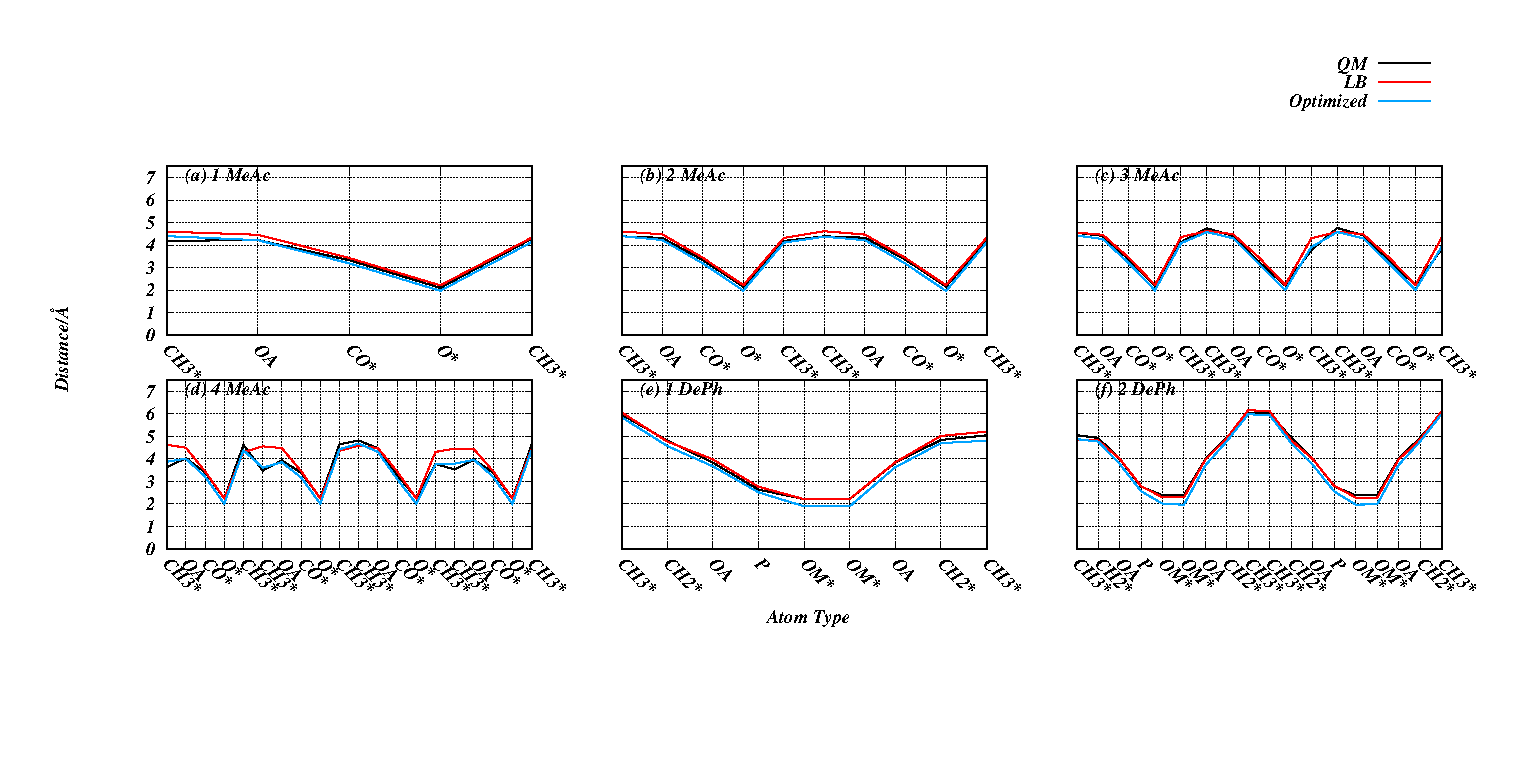
\includegraphics[width=0.8\textheight]{figure_s1.eps}
\end{sidewaysfigure}
\clearpage
\begin{table}
    \caption{Nelder--Meade constraints. These values were used to constrain the parameter search space during the NM--optimization.}
    \label{tab:constraints}
    {\tiny
    \begin{tabularx}{\textwidth}{X|X|X|X|X|X|X|X|X|X|}
	        &\tbxmulticol{2}{X|}{NA-CH3}&\tbxmulticol{2}{X|}{NA-CH2}&\tbxmulticol{2}{X|}{NA-CO*}&\tbxmulticol{2}{X|}{NA-OA,-OM*,-O*,-P}&Additional Constraints\\\hline
		&Min&Max&Min&Max&Min&Max&Min&Max&N/A\\\hline
	\sigmaij (nm)&0.2&0.5&0.2&0.5&0.2&0.5&0.2&0.5&$\sigma_{ij}^{\text{NA-OM*}}
        \leq \sigma_{ij}^{\text{NA-P}}$ \\\hline
	\epsilonij (kJ/mol) &0&0.79&0&0.81&0&0.83&0.05&7&N/A\\\hline
    \end{tabularx}
    }
\end{table}
\clearpage
\begin{figure}[htb]
    \caption{ Lipid chain deuterium order parameters. $S_{CD}$s are computed for each carbon
        for the chains Sn1 (a) and Sn2 (b), starting at the second carbon in the chain. We see that the optmized system is still showing significant ordering in the lipid
    chains as a result of ion binding; however, the ordering is less pronounced than in the system simulated with LB rules, 
    and is closer to that of the simulation without salt. This
result corresponds with the smaller bilayer thickness in the optimized system.
}
    \label{fig:op}
    %\includegraphics[width=\textwidth,trim=-3cm 0 0 0]{chainorder.eps}
%    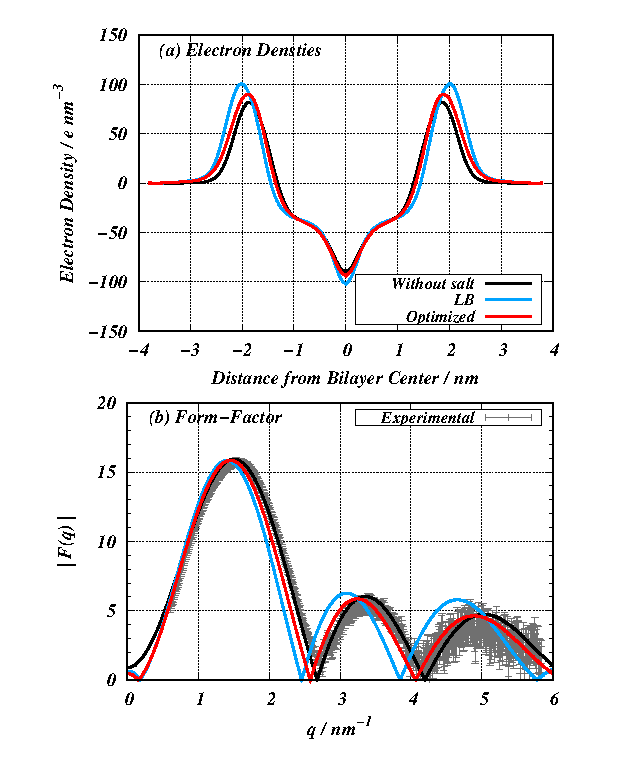
\includegraphics[width=\textwidth,trim=-3cm 0 0 0]{figure_4.eps}
    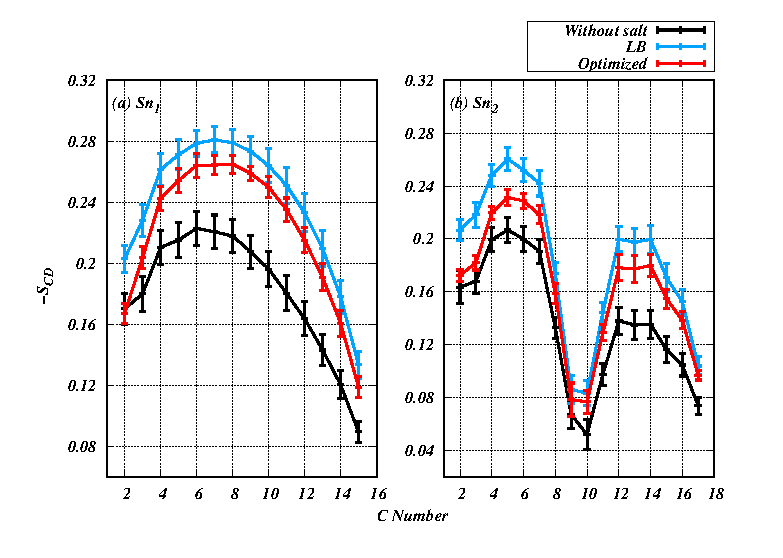
\includegraphics[width=\textwidth,trim=-3cm 0 0 0]{figure_s2.eps}
\end{figure}
\clearpage
\begin{figure}
    \caption{ Electrostatic potential as a function of distance from bilayer center. The optimized
cross terms yield a small change in the location of the peak of the potential in the
bilayer simulated with optimized cross terms, as well as the loss of the valley behind the peak.
}
    \label{fig:potential}
    %\includegraphics[width=\textwidth,trim=-3cm 0 0 0]{potential.eps}
    %\includegraphics[width=\textwidth,trim=-3cm 0 0 0]{figure_9.eps}
    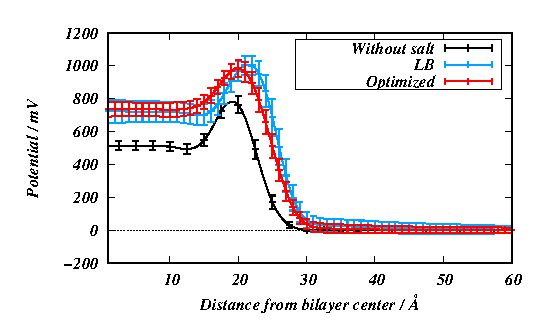
\includegraphics[width=\textwidth,trim=-3cm 0 0 0]{figure_s3.eps}
\end{figure}
\clearpage
\begin{figure}
    \caption{ Poisson-Boltzmann theory predictions and simulation results. (a) shows a snapshot of the 
system simulated with optimized cross terms, translated
to center the solvent occupied region. Water has been hidden
for clarity. (b) and (d)
    show the number density of ions in the solvent occupied region of the box. 
    (c) and (e) show the corresponding electrostatic potential in solvent.
    We illustrate theoretical predictions as solid lines, with corresponding 
    simulation results as points with error bars. Red vertical lines denote the \emph{hydration boundary} of the lipid bilayer. 
    \cl density data is used for fitting in both systems. 
}
    \label{fig:gouy}
    %\includegraphics[width=\textwidth,trim=0 0 0 0]{gouy.eps}
    %\includegraphics[width=\textwidth,trim=0 0 0 0]{figure_10.eps}
    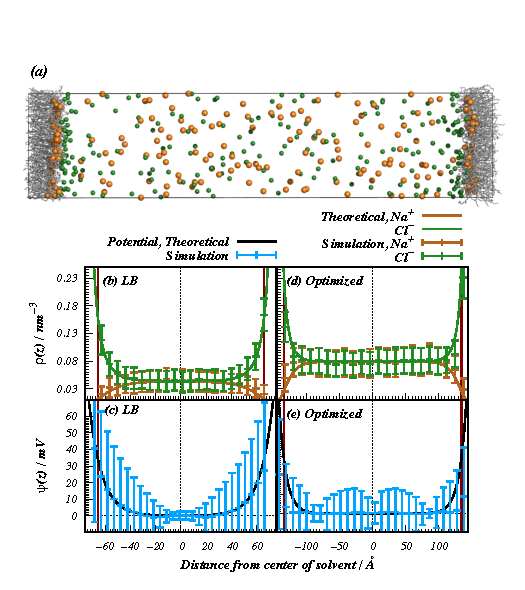
\includegraphics[width=\textwidth,trim=0 0 0 0]{figure_s4.eps}
\end{figure}

\end{document}
